\documentclass[12pt]{article}
\usepackage{amsmath, amssymb, amsfonts}
\usepackage{graphicx}
\usepackage{hyperref}
\usepackage{geometry}
\geometry{margin=1in}

\title{LAB NOTES : QRT Challenge 2025}
\author{Corentin C. L. Laudicina}
\date{}

\begin{document}

\maketitle

\section{Introduction}
Survival analysis refers to the study of time-to-event data. The \textit{event} of interest is often death, failure, or relapse in medical studies, but may correspond to other domains (e.g., machine failure, customer churn, etc.).

Unlike standard regression problems, survival data is often subject to \textit{censoring}, meaning that for some observations we only know a lower bound on the survival time.

\section{Survival and Hazard Functions}

Let $ T $ be a non-negative random variable representing the time to an event. Define:

\begin{itemize}

  \item The \textbf{survival function}:
  \begin{equation}
    S(t) = \mathbb{P}(T > t) = 1 - \mathrm{CDF}(t)
  \end{equation}
  where $\mathrm{CDF}(t)$ is the cumulative distribution function associated with the random variable $T$. The survival function $S(t)$ gives the probability that the event has not yet occurred by time $t$. We straightforwardly have the following limits: $S(t=0) = 1$, $S(t=\infty) = 0$ and also $S(t)$ is non-increasing. 
  \item The \textbf{hazard function}:
  \begin{equation}
    h(t) = \lim_{\Delta t \to 0} \frac{\mathbb{P}(t \leq T < t + \Delta t \mid T \geq t)}{\Delta t} = \frac{f(t)}{S(t)}
  \end{equation}
  where $f(t)= \partial_t \mathrm{CDF}(t)$ is the probability density function.
  \item The \textbf{cumulative hazard function} can be defined as:
  \begin{equation}
    H(t) = \int_0^t \mathrm{d}\tau h(\tau) = -\log S(t)
  \end{equation}
 and can be related to $h(t)$ via $h(t) = \partial_t H(t)$. 
  \item We can write the survival function $S(t)$ in terms of the hazard function $H(t)$
		\begin{equation}
			S(t) = e^{-H(t)} = e^{-\int_0^t\mathrm{d}\tau h(\tau)}
		\end{equation}
	From a physics perspective, we associate $S(t)$ with a Boltzmann weight and $h(t)$ to a Hamiltonian density. We therefore have one survival function 
\end{itemize}

\section{Censoring in Survival Analysis}

In survival analysis, the primary goal is to model the \emph{time until an event occurs}, such as death, relapse, or failure. However, in many real-world scenarios, we may not observe the event for all subjects within the study period. This leads to the concept of \textbf{censoring}, where the full survival time is only partially known.

\subsection{Types of Censoring}

\paragraph{1. Right-Censoring (Most Common)}
This occurs when the event of interest has not been observed by the end of the observation period. The only information we have is that the true event time exceeds the observed time.

\begin{itemize}
  \item \textbf{Example:} A patient is still alive at the end of the study or is lost to follow-up.
\end{itemize}

Let $ T $ be the true event time and $ C $ the censoring time. We observe:
\begin{equation}
\tilde{T} = \min(T, C), \qquad \delta = 
\begin{cases}
1 & \text{if } T \leq C \quad \text{(event observed)} \\
0 & \text{if } T > C \quad \text{(censored)}
\end{cases}
\end{equation}
Here, $ \delta $ is the \textbf{event indicator}, and $ \tilde{T} $ is the observed time.

\paragraph{2. Left-Censoring}
The event has occurred before the subject enters the study, but the exact time is unknown.

\begin{itemize}
  \item \textbf{Example:} A subject is found HIV-positive at their first screening, but the time of infection is unknown.
\end{itemize}

\paragraph{3. Interval-Censoring}
The event occurs within a known time interval, but the exact time is not observed.

\begin{itemize}
  \item \textbf{Example:} A machine is found broken between two maintenance checks, but we don’t know exactly when it failed.
\end{itemize}

\subsection{Importance of Censoring}

Censoring introduces incomplete data and, if not handled correctly, can bias the analysis. Standard techniques assume \emph{non-informative censoring}, meaning that the reason for censoring is independent of the true survival time.

Common methods to handle censoring include:
\begin{itemize}
  \item \textbf{Kaplan-Meier estimator:} Non-parametric estimator of the survival function.
  \item \textbf{Cox Proportional Hazards model:} Uses partial likelihood to account for censoring.
  \item \textbf{IPCW (Inverse Probability of Censoring Weights):} Adjusts evaluation metrics like the C-index to handle censoring.
\end{itemize}

\subsection{Assumption: Non-informative Censoring}

Most survival models rely on the assumption that censoring is independent of the outcome:
\begin{equation}
\mathbb{P}(C > t \mid T = t) = \mathbb{P}(C > t)
\end{equation}
If this assumption is violated, estimates may be biased, and more advanced techniques must be considered.

\section{Cox Proportional Hazards Model}

The Cox Proportional Hazards (PH) Model is a semi-parametric model used in survival analysis to investigate the effect of covariates on the time to a specific event, such as death or failure. It is widely used due to its flexibility and interpretability.

\subsection{Hazard Function}

The hazard function $h(t \mid \mathbf{x})$ gives the instantaneous rate at which the event occurs at time $t$, given that the individual has survived up to time $t$. In the Cox model, it is modeled as:
\begin{equation}
h(t \mid \mathbf{x}) = h_0(t) \exp(\mathbf{x}^\top \boldsymbol{\beta})
\end{equation}
where:
\begin{itemize}
  \item $h_0(t)$ is the \textbf{baseline hazard function}, common to all individuals.
  \item $\mathbf{x} \in \mathbb{R}^d$ is the covariate vector.
  \item $\boldsymbol{\beta} \in \mathbb{R}^d$ are the regression coefficients.
\end{itemize}

\subsection{Interpretation}

The model assumes that the covariates have a multiplicative effect on the hazard and that this effect is constant over time. That is:
\begin{equation}
\frac{h(t \mid \mathbf{x}_1)}{h(t \mid \mathbf{x}_2)} = \exp\left[(\mathbf{x}_1 - \mathbf{x}_2)^\top \boldsymbol{\beta}\right]
\end{equation}
This means the ratio of hazards between two individuals does not depend on time (proportional hazards assumption).

\subsection{Estimation via Partial Likelihood}

The Cox model does not require estimation of $h_0(t)$. Instead, it uses the \textbf{partial likelihood}, which considers only the ordering of events:
\begin{equation}
\mathcal{L}(\boldsymbol{\beta}) = \prod_{i \in \mathcal{D}} \frac{\exp(\mathbf{x}_i^\top \boldsymbol{\beta})}{\sum_{j \in \mathcal{R}(t_i)} \exp(\mathbf{x}_j^\top \boldsymbol{\beta})}
\end{equation}
where:
\begin{itemize}
  \item $\mathcal{D}$ is the set of individuals who experienced the event.
  \item $\mathcal{R}(t_i)$ is the risk set at time $t_i$ (all individuals still under observation at time $t_i$).
\end{itemize}

\subsection{Censoring}

The Cox model handles \textbf{right-censored} data naturally. For censored individuals, the partial likelihood simply excludes their contribution at the time of censoring.

\subsection{Advantages}

\begin{itemize}
  \item Does not assume a parametric form for $h_0(t)$.
  \item Easily extended to handle time-dependent covariates.
  \item Interpretability via hazard ratios.
\end{itemize}

\subsection{Limitations}

\begin{itemize}
  \item Assumes proportional hazards.
  \item May perform poorly with high-dimensional or highly correlated features.
  \item Cannot model complex, non-linear interactions directly without basis expansions or neural extensions.
\end{itemize}

\subsection{Extensions}

\begin{itemize}
  \item \textbf{Time-varying Cox models}: allow $\mathbf{x}(t)$ to change over time.
  \item \textbf{DeepSurv}: a neural network extension of CoxPH that replaces the linear term $\mathbf{x}^\top \boldsymbol{\beta}$ with a non-linear function.
\end{itemize}
\section{Model Evaluation}
Common evaluation metric: the \textbf{concordance index (C-index)} — a generalization of AUC for survival data. It measures the proportion of all usable patient pairs whose predicted risks correctly order their survival times.

\section{Speculations \& Stat Phys Connection}

In survival analysis, the central quantity is the \textit{survival function} $ S(t) $, which gives the probability that an individual has survived up to time $ t $. This is related to the \textit{hazard rate} $ h(t) $ via:
\begin{equation}
S(t) = \exp\left(-\int_0^t h(\tau) \, d\tau \right) = \exp(-H(t))
\end{equation}
where $ H(t) $ is the cumulative hazard. This exponential form resembles the \textit{Boltzmann weight} in statistical mechanics:
\begin{equation}
P(E) = \frac{1}{Z} \exp(-\beta E)
\end{equation}
This suggests an analogy: interpret $ H(t) $ as an effective \textit{risk energy}, and $ S(t) $ as an unnormalized probability weight for survival—just like $ \exp(-\beta E) $ represents the likelihood of a microstate with energy $ E $ at inverse temperature $ \beta $.

\subsection{Latent Risk Space}

We model the survival of each individual as a function of a latent risk representation. Let $t$ denote time, and let each patient $i$ be characterized by a latent feature vector $\mathbf{z}_i$ in some risk space. The survival function for patient $i$ is then modeled as
$$
S_i(t) = \exp\left(-E_i(\mathbf{z}_i, t)\right),
$$
where $E_i(\mathbf{z}_i, t)$ can be interpreted as a cumulative hazard, or "risk energy" associated with patient $i$ up to time $t$.

This expression is analogous to a Boltzmann weight $\exp(-\beta E)$ in statistical physics, where higher energy corresponds to lower probability. In our context, a high-risk individual has larger $E_i$ and thus lower survival probability $S_i(t)$.

To consider the full population of $N$ patients, we define the population survival mass as
$$
Z(t) = \sum_{i=1}^{N} S_i(t) = \sum_{i=1}^{N} \exp\left(-E_i(\mathbf{z}_i, t)\right).
$$
This plays a role similar to the partition function in statistical mechanics, summing over survival probabilities of all individuals.

In a continuous formulation, where patients are drawn from a density $p(\mathbf{z})$ over the latent space, we can write
$$
Z(t) = \int d\mathbf{z} \, p(\mathbf{z}) \, \exp\left(-E(\mathbf{z}, t)\right).
$$

This integral formulation corresponds to computing a population-level average survival. The function $Z(t)$ encodes the overall risk distribution across the population, and we may define a time-dependent survival-based free energy via
$$
F(t) = -\log Z(t),
$$
analogous to thermodynamic free energy. This quantity captures the collective risk landscape at time $t$.

\subsection{Latent Risk Partition Function (Per-Patient)}

We now consider a per-patient formulation of survival using an analogy with statistical mechanics. Each patient $ i $ is associated with a latent variable vector $ \mathbf{z}_i $, learned for example through an autoencoder.
We define a patient-specific partition function:
\begin{equation}
Z_i(t) = \int d\mathbf{z} \; p_i(\mathbf{z}) \; e^{-E(\mathbf{z}, t)},
\end{equation}
where:
\begin{itemize}
    \item $ p_i(\mathbf{z}) $ is a (possibly learned) probability distribution over latent features for patient $ i $,
    \item $ E(\mathbf{z}, t) $ is an effective risk energy at time $ t $, which plays the role of a time-dependent Hamiltonian.
\end{itemize}

The per-patient survival function is then given by:
\begin{equation}
S_i(t) = \frac{Z_i(t)}{Z_i(0)},
\end{equation}
which satisfies $ S_i(0) = 1 $ by construction. Intuitively, the higher the energy associated with latent state $ \mathbf{z} $, the lower its contribution to survival at time $ t $.

This framework allows us to interpret survival as a weighted average over latent risk paths, with weights defined by the Boltzmann-like factor $ e^{-E(\mathbf{z}, t)} $. If $ E(\mathbf{z}, t) $ increases with time, survival decays.

\clearpage
\section{Analysis of the Dataset}

\subsection{Feature Distribution}
To investigate potential dataset shift, we compared the distributions of key clinical features between the training and inference (test) sets, shown in Fig.~\ref{fig:feature_distributions}. Most features--such as BM-BLAST, WBC, and PLT--showed consistent distributions across both sets, suggesting stable input statistics. However, two notable exceptions were observed: the HB (hemoglobin) feature displayed a slight distributional shift, and the has-TP53-mutation binary feature had a markedly higher frequency in the test set (~26\%) compared to the training set (~11\%). Since TP53 mutations are strongly associated with poor prognosis in hematologic malignancies, this imbalance could partially explain reduced generalization performance.

\begin{figure}[h]
\centering
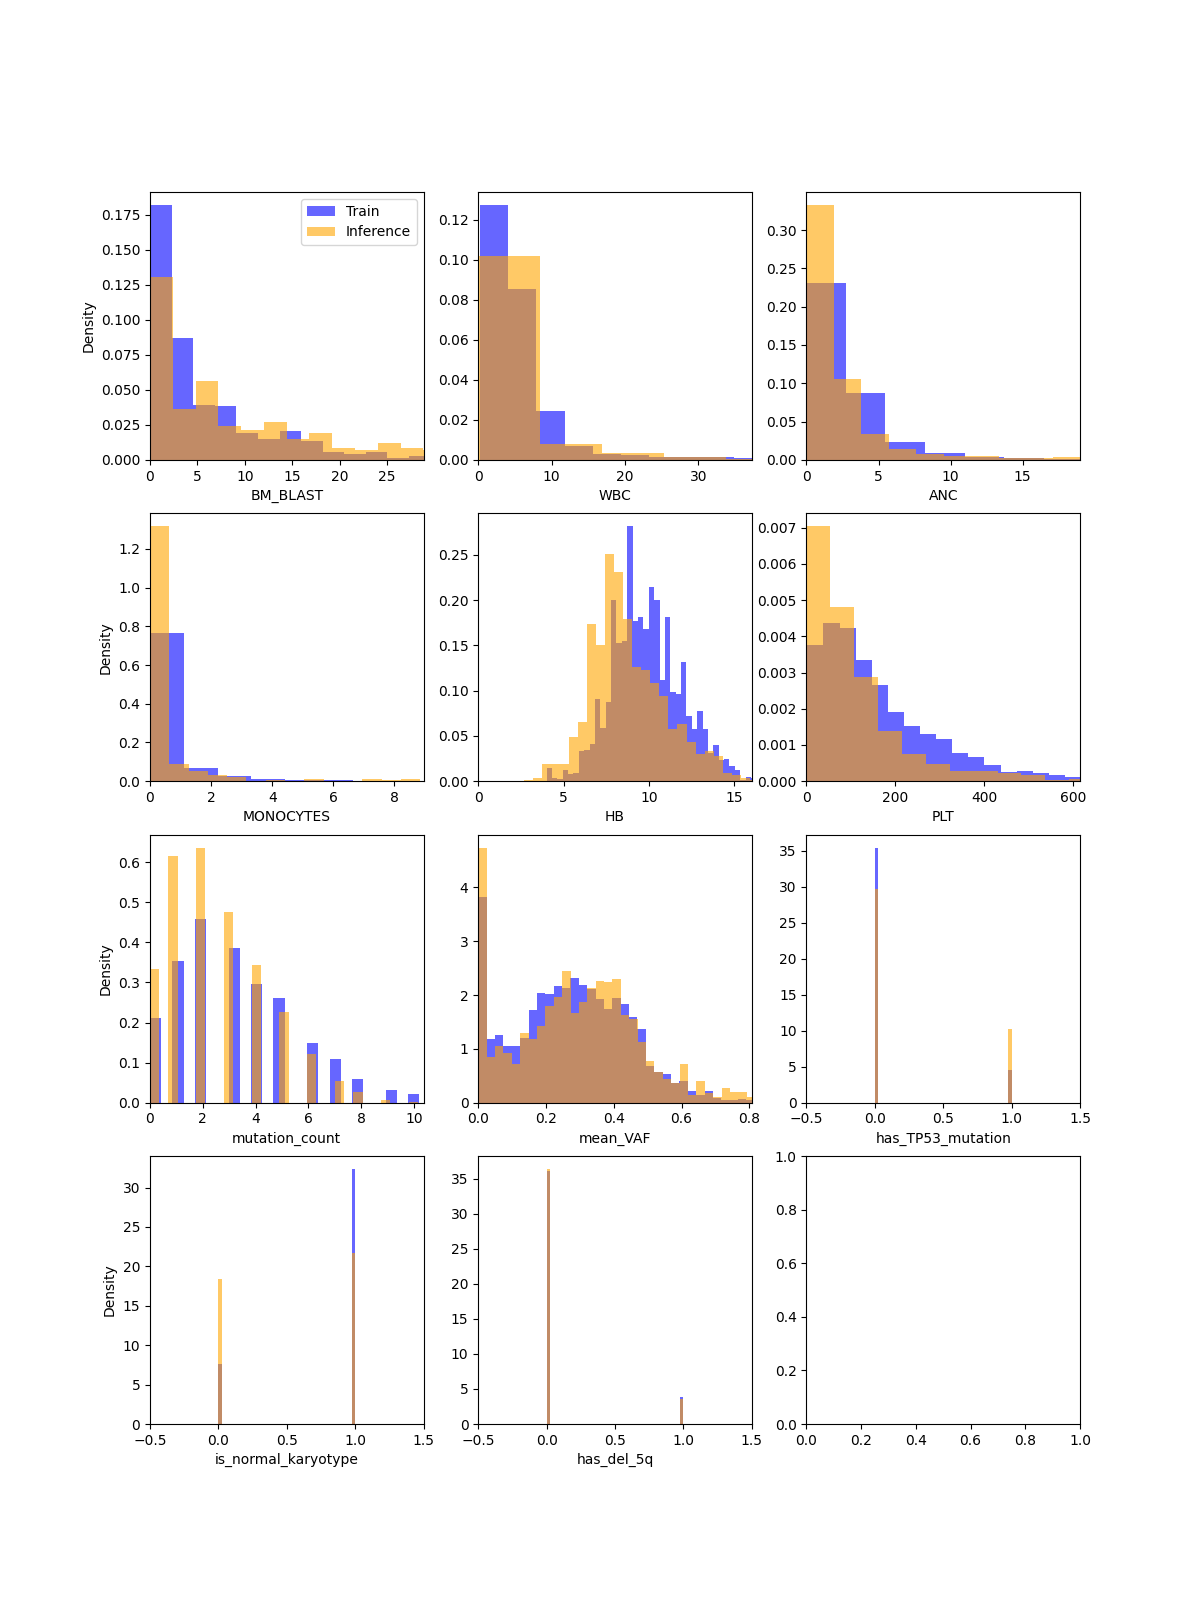
\includegraphics[width=\linewidth]{Figures/feature_distributions.png}
\caption{Feature Distributions of Training and Inference sets}
\label{fig:feature_distributions}
\end{figure}

The mutation and cytogenetic data in our dataset is really sparse — most patients only have a few mutations or chromosomal changes, and there are a huge number of possible features overall. This makes it hard for our models to learn anything meaningful from them directly. So instead, we use autoencoders to compress this information into a smaller number of continuous features. The idea is to keep the important patterns while ignoring the noise. These compressed features (embeddings) are then used in our survival models, which makes them easier to train and hopefully better at generalizing.

We analyzed the autoencoder embeddings derived from binary representations of mutation (see Fig.~\ref{fig:mut_embed_distribution}) and cytogenetic data (see Fig.~\ref{fig:cyto_embed_distribution}). These two sources are highly sparse and high-dimensional, mainly because of the complex and diverse nature of genetic changes in blood cancers. Mutation embeddings appeared to follow similar distributions in both the training and test sets. However, the cytogenetic embeddings were noticeably different, likely due to the rare and varied nature of chromosomal abnormalities, which often occur in only a few patients. This mismatch suggested that the autoencoder might be overfitting to specific patterns in the training data. We have also performed tests where the inference sets were also included in the autoencoding, with little improvements. As a result, we suggest not to make use of the full cytogenetic embeddings and to instead use simple binary features indicating known high-risk abnormalities (such as deletion of chromosome 5q or loss of chromosome 7). This has shown to increase generalization performance across the board for the various models considered. 

To understand the cytogenetic data further, we also performed a PCA analysis on the cytogenetic data. the results support our hypothesis that the data is extremely sparse. As shown in Fig.~\ref{cytogenetics_pca}, the cumulative explained variance of the first 8 components reaches only about 35\%, meaning that only a third of the variance in the data can be captured by these components. This suggests that it is difficult to compress the cytogenetic dataset into a lower-dimensional subspace, due to its high sparsity and complexity.

\begin{figure}[h]
\centering
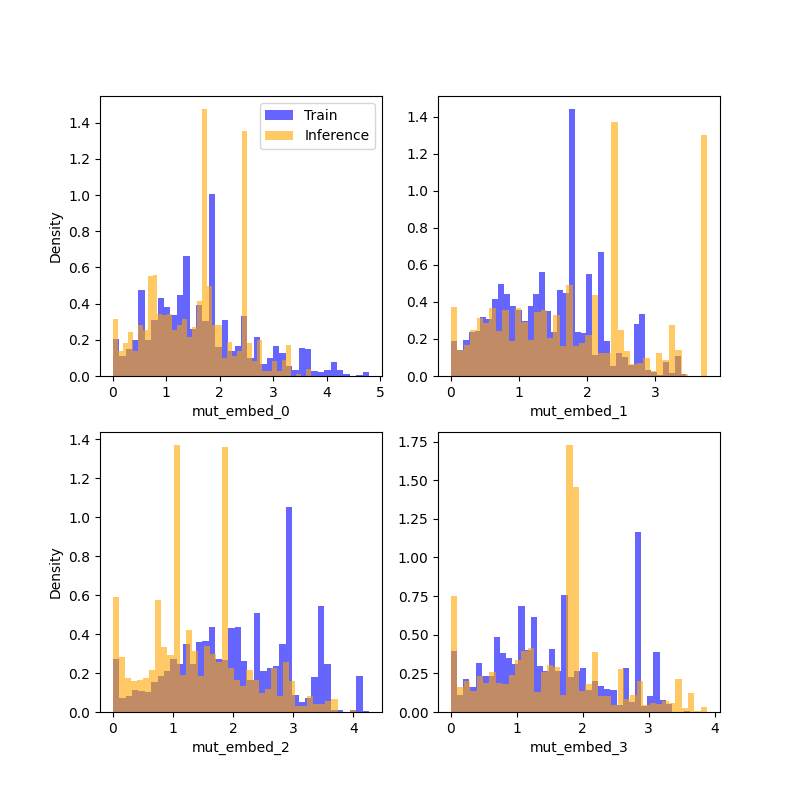
\includegraphics[width=0.75\linewidth]{Figures/mut_embed_distribution.png}
\caption{Feature Distributions of the encoding of the mutation data of Training and Inference sets}
\label{fig:mut_embed_distribution}
\end{figure}

\begin{figure}[h]
\centering
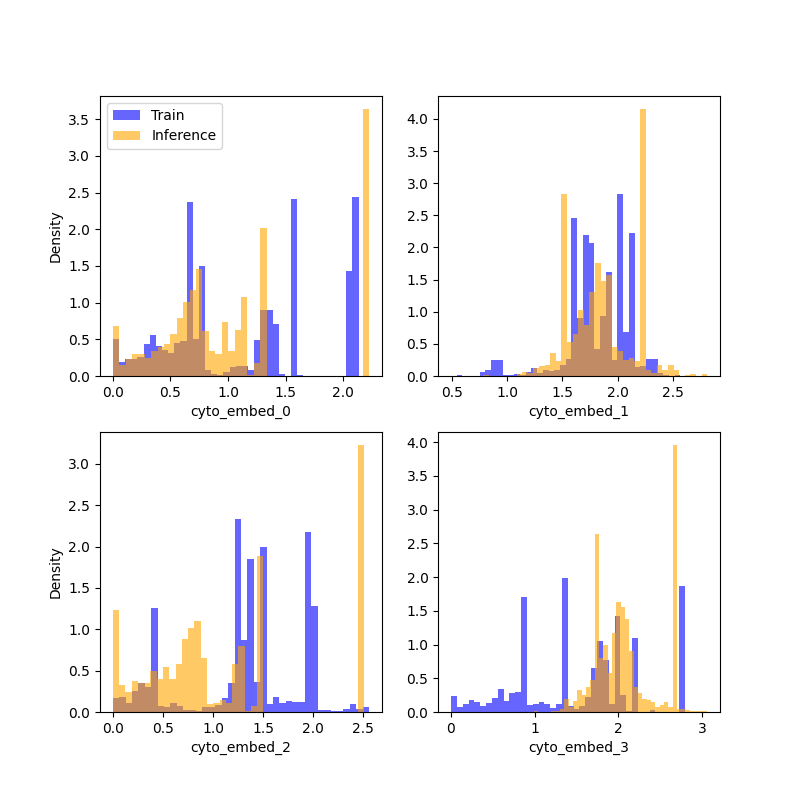
\includegraphics[width=0.75\linewidth]{Figures/cyto_embed_distribution.png}
\caption{Feature Distributions of the encoding of the cytogenetic data in Training of Inference sets}
\label{fig:cyto_embed_distribution}
\end{figure}

\begin{figure}[h]
\centering
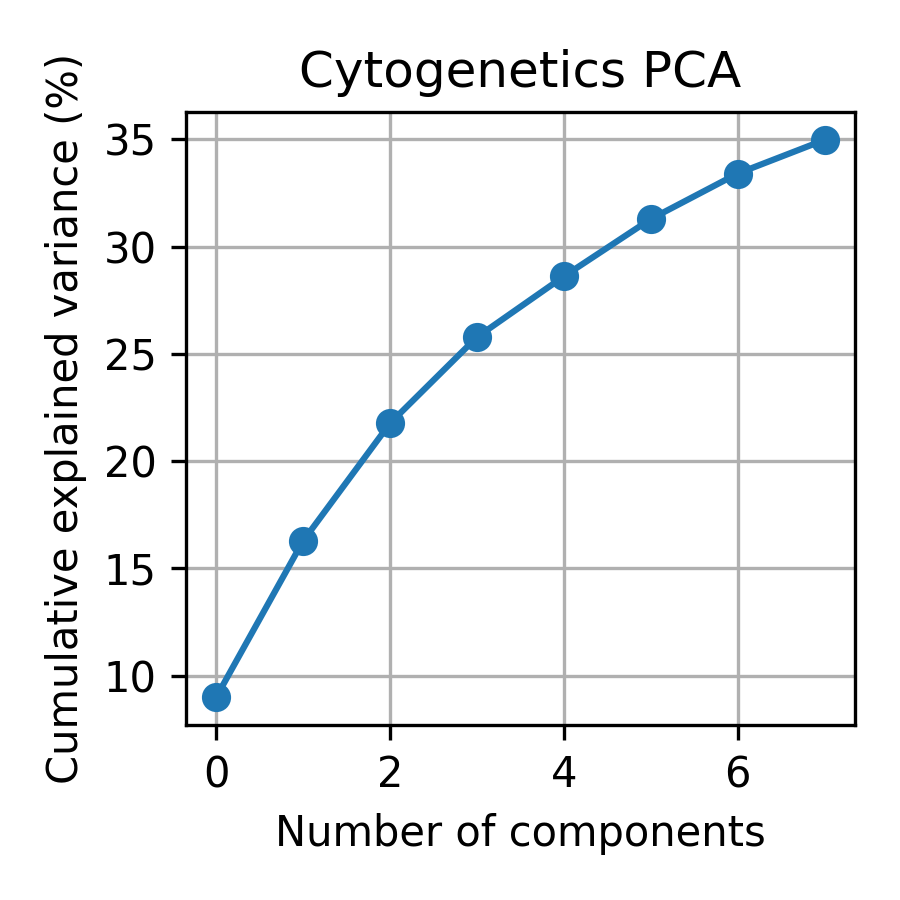
\includegraphics[width=0.5\linewidth]{Figures/cytogenetics_pca.png}
\caption{Principal Components for Cytogenetic Data}
\label{fig:cytogenetics_pca}
\end{figure}





\end{document}